%%%%%%%%%%%%%%%%%%%%%%%%%%%%%%%%%%%%%%%%%%%%%%%%%%%%%%%%%%%%%%%%%%%%%%%%%%%
%% This file is part of the book
%%
%% Algorithmic Graph Theory
%% http://code.google.com/p/graph-theory-algorithms-book/
%%
%% Copyright (C) 2009, 2010, 2011 Minh Van Nguyen <nguyenminh2@gmail.com>
%%
%% See the file COPYING for copying conditions.
%%%%%%%%%%%%%%%%%%%%%%%%%%%%%%%%%%%%%%%%%%%%%%%%%%%%%%%%%%%%%%%%%%%%%%%%%%%

\documentclass{article}

\usepackage{subfigure}
\usepackage{tikz}
\usetikzlibrary{external}
\usetikzlibrary{trees}
\tikzexternalize{binomial-heap-extract}

\begin{document}

\begin{figure}
\subfigure[]{
\scriptsize
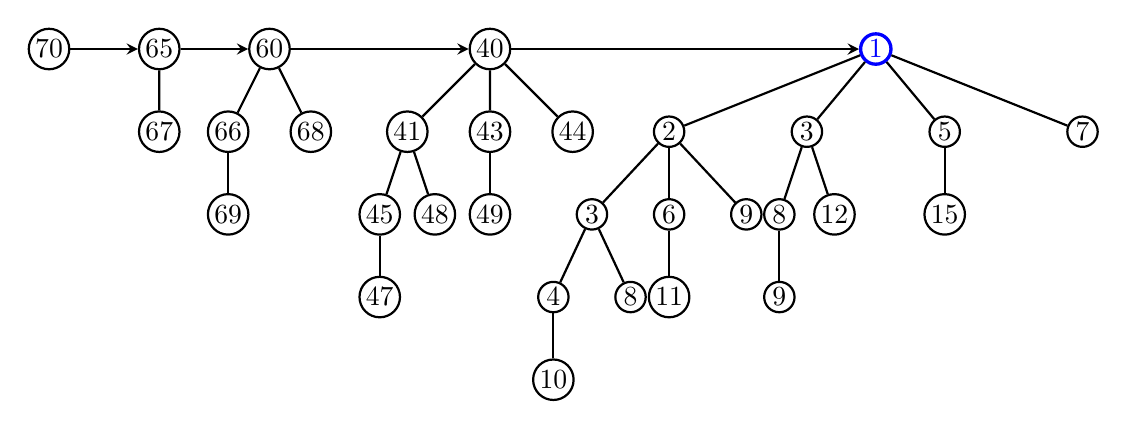
\begin{tikzpicture}
[-,thick,%
  every node/.style={shape=circle,inner sep=1pt,draw,thick},%
  scale=0.7]
\node (70) at (0,0) {$70$};
%%
\node (65) at (2,0) {$65$}
  child {node {$67$}};
%%
\node (60) at (4,0) {$60$}
  child {node {$66$}
    child {node {$69$}}
  }
  child {node {$68$}};
%%
\node (40) at (8,0) {$40$}
  child {node {$41$}
      [sibling distance=1cm]
    child {node {$45$}
      child {node {$47$}}
    }
    child {node {$48$}}
  }
  child {node {$43$}
    child {node {$49$}}
  }
  child {node {$44$}};
%%
\node[blue,very thick] (1) at (15,0) {$1$}
  [sibling distance=2.5cm]
  child {node {$2$}
    [sibling distance=1.4cm]
    child {node {$3$}
      child {node {$4$}
        child {node {$10$}}
      }
      child {node {$8$}}
    }
    child {node {$6$}
      child {node {$11$}}
    }
    child {node {$9$}}
  }
  child {node {$3$}
    [sibling distance=1cm]
    child {node {$8$}
      child {node {$9$}}
    }
    child {node {$12$}}
  }
  child {node {$5$}
    [sibling distance=1cm]
    child {node {$15$}}
  }
  child {node {$7$}};
\path
\foreach \startNode/\endNode in {70/65, 65/60, 60/40, 40/1}
{
  (\startNode) edge[->,>=stealth,thick] (\endNode)
};
\end{tikzpicture}
}
%%
%%
\subfigure[]{
\scriptsize
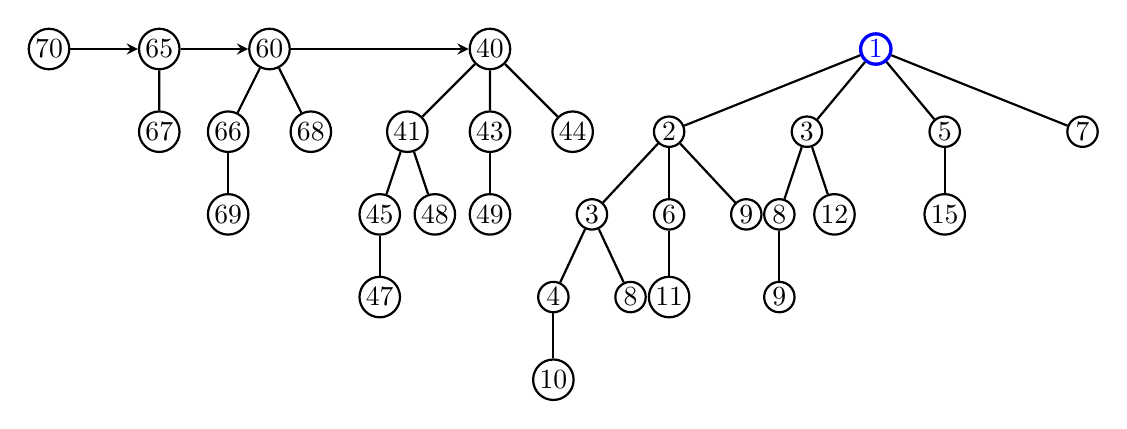
\begin{tikzpicture}
[-,thick,%
  every node/.style={shape=circle,inner sep=1pt,draw,thick},%
  scale=0.7]
\node (70) at (0,0) {$70$};
%%
\node (65) at (2,0) {$65$}
  child {node {$67$}};
%%
\node (60) at (4,0) {$60$}
  child {node {$66$}
    child {node {$69$}}
  }
  child {node {$68$}};
%%
\node (40) at (8,0) {$40$}
  child {node {$41$}
    [sibling distance=1cm]
    child {node {$45$}
      child {node {$47$}}
    }
    child {node {$48$}}
  }
  child {node {$43$}
    child {node {$49$}}
  }
  child {node {$44$}};
%%
\node[blue,very thick] at (15,0) {$1$}
  [sibling distance=2.5cm]
  child {node {$2$}
    [sibling distance=1.4cm]
    child {node {$3$}
      child {node {$4$}
        child {node {$10$}}
      }
      child {node {$8$}}
    }
    child {node {$6$}
      child {node {$11$}}
    }
    child {node {$9$}}
  }
  child {node {$3$}
    [sibling distance=1cm]
    child {node {$8$}
      child {node {$9$}}
    }
    child {node {$12$}}
  }
  child {node {$5$}
    [sibling distance=1cm]
    child {node {$15$}}
  }
  child {node {$7$}};
\path
\foreach \startNode/\endNode in {70/65, 65/60, 60/40}
{
  (\startNode) edge[->,>=stealth,thick] (\endNode)
};
\end{tikzpicture}
}
%%
%%
\subfigure[]{
\scriptsize
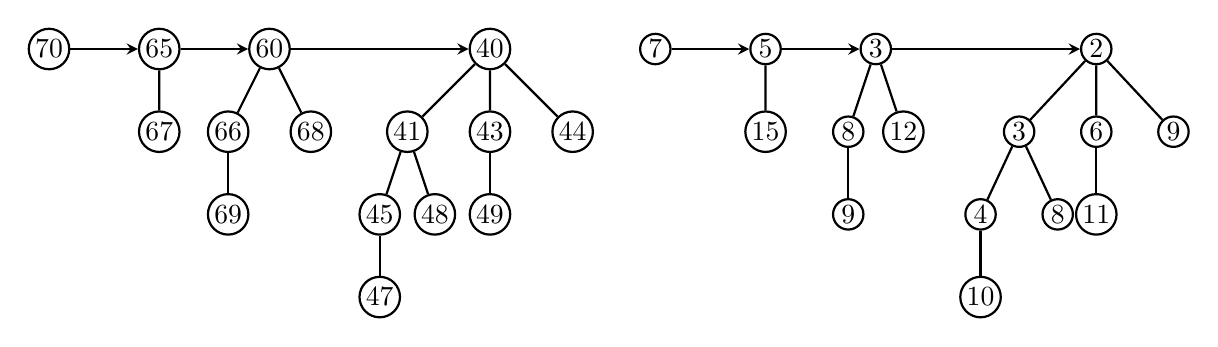
\begin{tikzpicture}
[-,thick,%
  every node/.style={shape=circle,inner sep=1pt,draw,thick},%
  scale=0.7]
\node (70) at (0,0) {$70$};
%%
\node (65) at (2,0) {$65$}
  child {node {$67$}};
%%
\node (60) at (4,0) {$60$}
  child {node {$66$}
    child {node {$69$}}
  }
  child {node {$68$}};
%%
\node (40) at (8,0) {$40$}
  child {node {$41$}
    [sibling distance=1cm]
    child {node {$45$}
      child {node {$47$}}
    }
    child {node {$48$}}
  }
  child {node {$43$}
    child {node {$49$}}
  }
  child {node {$44$}};
%%
\node (7) at (11,0) {$7$};
%%
\node (5) at (13,0) {$5$}
  child {node {$15$}};
%%
\node (3) at (15,0) {$3$}
  [sibling distance=1cm]
  child {node {$8$}
    child {node {$9$}}
  }
  child {node {$12$}};
%%
\node (2) at (19,0) {$2$}
  [sibling distance=1.4cm]
  child {node {$3$}
    child {node {$4$}
      child {node {$10$}}
    }
    child {node {$8$}}
  }
  child {node {$6$}
    child {node {$11$}}
  }
  child {node {$9$}};
\path
\foreach \startNode/\endNode in {70/65, 65/60, 60/40}
{
  (\startNode) edge[->,>=stealth,thick] (\endNode)
};
\path
\foreach \startNode/\endNode in {7/5, 5/3, 3/2}
{
  (\startNode) edge[->,>=stealth,thick] (\endNode)
};
\end{tikzpicture}
}
%%
%%
\subfigure[]{
\scriptsize
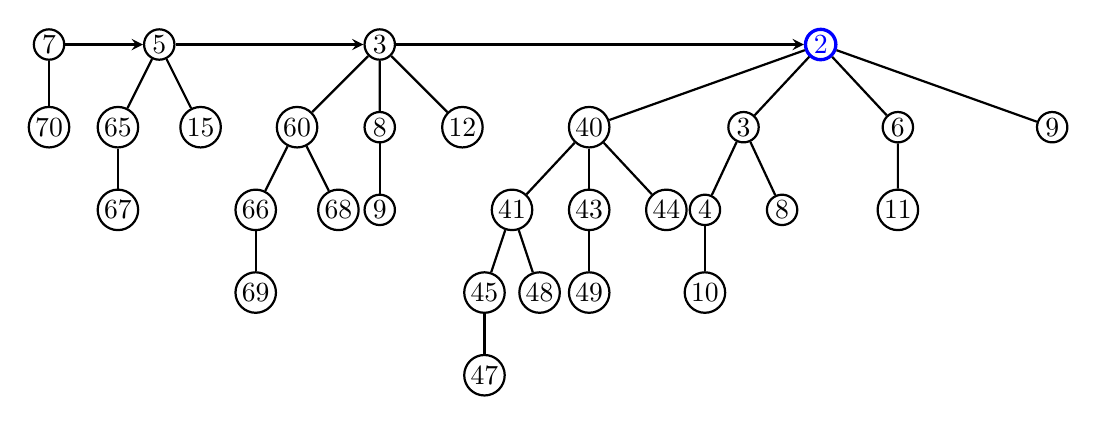
\begin{tikzpicture}
[-,thick,%
  every node/.style={shape=circle,inner sep=1pt,draw,thick},%
  scale=0.7]
\node (7) at (0,0) {$7$}
  child {node {$70$}};
%%
\node (5) at (2,0) {$5$}
  child {node {$65$}
    child {node {$67$}}
  }
  child {node {$15$}};
%%
\node (3) at (6,0) {$3$}
  child {node {$60$}
    child {node {$66$}
      child {node {$69$}}
    }
    child {node {$68$}}
  }
  child {node {$8$}
    child {node {$9$}}
  }
  child {node {$12$}};
%%
\node[blue,very thick] (2) at (14,0) {$2$}
  [sibling distance=2.8cm]
  child {node {$40$}
    [sibling distance=1.4cm]
    child {node {$41$}
      [sibling distance=1cm]
      child {node {$45$}
        child {node {$47$}}
      }
      child {node {$48$}}
    }
    child {node {$43$}
      child {node {$49$}}
    }
    child {node {$44$}}
  }
  child {node {$3$}
    [sibling distance=1.4cm]
    child {node {$4$}
      child {node {$10$}}
    }
    child {node {$8$}}
  }
  child {node {$6$}
    child {node {$11$}}
  }
  child {node {$9$}};
\path
\foreach \startNode/\endNode in {7/5, 5/3, 3/2}
{
  (\startNode) edge[->,>=stealth,thick] (\endNode)
};
\end{tikzpicture}
}
\end{figure}

\end{document}
